\section{The Case of Small Spins}
While for many phenomena of the Dicke model it is useful and necessary to study large spin, some elementary effects are observable in the case of small spin ($j= 1/2, 1 ,\dots$) too.
More importantly, if the spin is small patterns can be found that are hidden in the larger spin cases.
Following the work of Müller et al. [?], It is possible to show that the level spacing distribution follows a well defined limit starting from the smallest spin of $1/2$ to arbitrarily large spin.
This allows a more quantitative approach to the question of integrability.
It is known that for an integrable case the level spacing distribution becomes \textcolor{red}{Poissonic} in the thermodynamic limit, while in the nonitegrable case it will approach a Wigner distribution [?].
As shown by Müller et al it is possible for the integrable case of the Dicke model ($\delta = 0, \alpha = 0$) to find a universal distribution function for arbitrary spin that describes the level spacing distribution and converges to a Poisson distribution in the limit of infinite spin length, at least for a specific set of parameters in which the coupling strength is relatively weak ($\gamma = 0.5$).

In the following paragraph I will try to generalize this method to the nonintegrable case, once for arbitrary $\delta$ and once for arbitrary alpha, while the other parameter remains zero.
What we first need are candidates of function sequence that converges to the Wigner distribution.
The simplest candidate would be
\begin{equation}
	p_n(x) = x \left(1-\frac{x^2}{n}\right)^n
\end{equation}
with the limit $\lim\limits_{n\rightarrow \infty} p_n(x) = x e^{-x^2}$ for $-1 \leq x \leq 1$.
Since the general density distribution found by Müller et al for the integrable case is only applicable for one specific set of parameters, here we will try to achieve the same, while a general analytical formula suitable for arbitrary parameters is seemingly impossible to find.
%Peres lattices for small spin
The emergence of nonintegrability can also be seen in the spectrum of small spin if we apply the method of Peres lattices in this regime.
Here the transition from organized lattices to chaotic order is better observable, since the lattices are well separated strands or bands of points, so crossing or interaction of any kind between them is a sign of nonitegrability.
The reason for the bands is the existence of some other conserved quantity besides the energy in this case the total number of excitations. 
If the parity is conserved we should see two independent sets of bands that are independent even in the nonitegrable case but in the small spin case it might be difficult to distinguish between crossing and avoided crossing of bands, since they are not continuous. 
It is also important to notice that, while fundamentally interchangeable, the specific form of the bands depends heavily on the choice of invariants.

%Method of Müller et al
The method that Müller et al. used to find the model for the energy spacing is a set of $n = 2j+1$ one dimensional lattices with incommensurable spacings. 
Calculating the spacing distribution of the superposition of those lattices yields a reasonably good approximation for the numerically determined spacing distribution of the spin boson model in the limit of small differences in the lattice constants.
That model is reasonable if we assume that the bands have almost equidistant spacing internally, which is a reasonable assumption, but only if small sections of the spectrum are considered.
The assumption of independent lattices for the different bands is justified by the integrability effect, so in the nonintegrable case such a model can not hold.
I have recreated the spacing distribution for several spin length in figure \ref{fig:hist_I0.5} for the integrable case.
Here it can be seen, that only for large spin the distribution matches the general formula
\begin{equation}
  p_n (x) = x \left( 1 - \frac{x}{n}\right)^n \label{eq:p_n-I}
\end{equation}
which was postulated by Müller et al. matches the dirstribution of the spacings to a agreeable level.
\begin{figure}[h]
  \centering
  % GNUPLOT: LaTeX picture with Postscript
\begingroup
  \makeatletter
  \providecommand\color[2][]{%
    \GenericError{(gnuplot) \space\space\space\@spaces}{%
      Package color not loaded in conjunction with
      terminal option `colourtext'%
    }{See the gnuplot documentation for explanation.%
    }{Either use 'blacktext' in gnuplot or load the package
      color.sty in LaTeX.}%
    \renewcommand\color[2][]{}%
  }%
  \providecommand\includegraphics[2][]{%
    \GenericError{(gnuplot) \space\space\space\@spaces}{%
      Package graphicx or graphics not loaded%
    }{See the gnuplot documentation for explanation.%
    }{The gnuplot epslatex terminal needs graphicx.sty or graphics.sty.}%
    \renewcommand\includegraphics[2][]{}%
  }%
  \providecommand\rotatebox[2]{#2}%
  \@ifundefined{ifGPcolor}{%
    \newif\ifGPcolor
    \GPcolortrue
  }{}%
  \@ifundefined{ifGPblacktext}{%
    \newif\ifGPblacktext
    \GPblacktexttrue
  }{}%
  % define a \g@addto@macro without @ in the name:
  \let\gplgaddtomacro\g@addto@macro
  % define empty templates for all commands taking text:
  \gdef\gplbacktext{}%
  \gdef\gplfronttext{}%
  \makeatother
  \ifGPblacktext
    % no textcolor at all
    \def\colorrgb#1{}%
    \def\colorgray#1{}%
  \else
    % gray or color?
    \ifGPcolor
      \def\colorrgb#1{\color[rgb]{#1}}%
      \def\colorgray#1{\color[gray]{#1}}%
      \expandafter\def\csname LTw\endcsname{\color{white}}%
      \expandafter\def\csname LTb\endcsname{\color{black}}%
      \expandafter\def\csname LTa\endcsname{\color{black}}%
      \expandafter\def\csname LT0\endcsname{\color[rgb]{1,0,0}}%
      \expandafter\def\csname LT1\endcsname{\color[rgb]{0,1,0}}%
      \expandafter\def\csname LT2\endcsname{\color[rgb]{0,0,1}}%
      \expandafter\def\csname LT3\endcsname{\color[rgb]{1,0,1}}%
      \expandafter\def\csname LT4\endcsname{\color[rgb]{0,1,1}}%
      \expandafter\def\csname LT5\endcsname{\color[rgb]{1,1,0}}%
      \expandafter\def\csname LT6\endcsname{\color[rgb]{0,0,0}}%
      \expandafter\def\csname LT7\endcsname{\color[rgb]{1,0.3,0}}%
      \expandafter\def\csname LT8\endcsname{\color[rgb]{0.5,0.5,0.5}}%
    \else
      % gray
      \def\colorrgb#1{\color{black}}%
      \def\colorgray#1{\color[gray]{#1}}%
      \expandafter\def\csname LTw\endcsname{\color{white}}%
      \expandafter\def\csname LTb\endcsname{\color{black}}%
      \expandafter\def\csname LTa\endcsname{\color{black}}%
      \expandafter\def\csname LT0\endcsname{\color{black}}%
      \expandafter\def\csname LT1\endcsname{\color{black}}%
      \expandafter\def\csname LT2\endcsname{\color{black}}%
      \expandafter\def\csname LT3\endcsname{\color{black}}%
      \expandafter\def\csname LT4\endcsname{\color{black}}%
      \expandafter\def\csname LT5\endcsname{\color{black}}%
      \expandafter\def\csname LT6\endcsname{\color{black}}%
      \expandafter\def\csname LT7\endcsname{\color{black}}%
      \expandafter\def\csname LT8\endcsname{\color{black}}%
    \fi
  \fi
    \setlength{\unitlength}{0.0500bp}%
    \ifx\gptboxheight\undefined%
      \newlength{\gptboxheight}%
      \newlength{\gptboxwidth}%
      \newsavebox{\gptboxtext}%
    \fi%
    \setlength{\fboxrule}{0.5pt}%
    \setlength{\fboxsep}{1pt}%
\begin{picture}(6802.00,9070.00)%
    \gplgaddtomacro\gplbacktext{%
      \csname LTb\endcsname%
      \put(594,7242){\makebox(0,0)[r]{\strut{}$0$}}%
      \put(594,7437){\makebox(0,0)[r]{\strut{}$0.2$}}%
      \put(594,7631){\makebox(0,0)[r]{\strut{}$0.4$}}%
      \put(594,7826){\makebox(0,0)[r]{\strut{}$0.6$}}%
      \put(594,8020){\makebox(0,0)[r]{\strut{}$0.8$}}%
      \put(594,8215){\makebox(0,0)[r]{\strut{}$1$}}%
      \put(594,8409){\makebox(0,0)[r]{\strut{}$1.2$}}%
      \put(726,7022){\makebox(0,0){\strut{}$0$}}%
      \put(1273,7022){\makebox(0,0){\strut{}$0.248175$}}%
      \put(1819,7022){\makebox(0,0){\strut{}$0.49635$}}%
      \put(2366,7022){\makebox(0,0){\strut{}$0.744526$}}%
      \put(2913,7022){\makebox(0,0){\strut{}$0.992701$}}%
    }%
    \gplgaddtomacro\gplfronttext{%
      \csname LTb\endcsname%
      \put(1865,8739){\makebox(0,0){\strut{}$j = 1/2$}}%
    }%
    \gplgaddtomacro\gplbacktext{%
      \csname LTb\endcsname%
      \put(3995,7242){\makebox(0,0)[r]{\strut{}$0$}}%
      \put(3995,7475){\makebox(0,0)[r]{\strut{}$0.5$}}%
      \put(3995,7709){\makebox(0,0)[r]{\strut{}$1$}}%
      \put(3995,7942){\makebox(0,0)[r]{\strut{}$1.5$}}%
      \put(3995,8176){\makebox(0,0)[r]{\strut{}$2$}}%
      \put(3995,8409){\makebox(0,0)[r]{\strut{}$2.5$}}%
      \put(4127,7022){\makebox(0,0){\strut{}$0$}}%
      \put(4674,7022){\makebox(0,0){\strut{}$0.2174$}}%
      \put(5220,7022){\makebox(0,0){\strut{}$0.4348$}}%
      \put(5767,7022){\makebox(0,0){\strut{}$0.6522$}}%
      \put(6314,7022){\makebox(0,0){\strut{}$0.8696$}}%
    }%
    \gplgaddtomacro\gplfronttext{%
      \csname LTb\endcsname%
      \put(5266,8739){\makebox(0,0){\strut{}$j = 1$}}%
    }%
    \gplgaddtomacro\gplbacktext{%
      \csname LTb\endcsname%
      \put(594,4975){\makebox(0,0)[r]{\strut{}$0$}}%
      \put(594,5142){\makebox(0,0)[r]{\strut{}$0.5$}}%
      \put(594,5308){\makebox(0,0)[r]{\strut{}$1$}}%
      \put(594,5475){\makebox(0,0)[r]{\strut{}$1.5$}}%
      \put(594,5642){\makebox(0,0)[r]{\strut{}$2$}}%
      \put(594,5809){\makebox(0,0)[r]{\strut{}$2.5$}}%
      \put(594,5975){\makebox(0,0)[r]{\strut{}$3$}}%
      \put(594,6142){\makebox(0,0)[r]{\strut{}$3.5$}}%
      \put(726,4755){\makebox(0,0){\strut{}$0$}}%
      \put(1273,4755){\makebox(0,0){\strut{}$0.206085$}}%
      \put(1819,4755){\makebox(0,0){\strut{}$0.41217$}}%
      \put(2366,4755){\makebox(0,0){\strut{}$0.618254$}}%
      \put(2913,4755){\makebox(0,0){\strut{}$0.824339$}}%
    }%
    \gplgaddtomacro\gplfronttext{%
      \csname LTb\endcsname%
      \put(1865,6472){\makebox(0,0){\strut{}$j = 3/2$}}%
    }%
    \gplgaddtomacro\gplbacktext{%
      \csname LTb\endcsname%
      \put(3995,4975){\makebox(0,0)[r]{\strut{}$0$}}%
      \put(3995,5105){\makebox(0,0)[r]{\strut{}$0.5$}}%
      \put(3995,5234){\makebox(0,0)[r]{\strut{}$1$}}%
      \put(3995,5364){\makebox(0,0)[r]{\strut{}$1.5$}}%
      \put(3995,5494){\makebox(0,0)[r]{\strut{}$2$}}%
      \put(3995,5623){\makebox(0,0)[r]{\strut{}$2.5$}}%
      \put(3995,5753){\makebox(0,0)[r]{\strut{}$3$}}%
      \put(3995,5883){\makebox(0,0)[r]{\strut{}$3.5$}}%
      \put(3995,6012){\makebox(0,0)[r]{\strut{}$4$}}%
      \put(3995,6142){\makebox(0,0)[r]{\strut{}$4.5$}}%
      \put(4127,4755){\makebox(0,0){\strut{}$0$}}%
      \put(4674,4755){\makebox(0,0){\strut{}$0.185581$}}%
      \put(5220,4755){\makebox(0,0){\strut{}$0.371162$}}%
      \put(5767,4755){\makebox(0,0){\strut{}$0.556743$}}%
      \put(6314,4755){\makebox(0,0){\strut{}$0.742324$}}%
    }%
    \gplgaddtomacro\gplfronttext{%
      \csname LTb\endcsname%
      \put(5266,6472){\makebox(0,0){\strut{}$j = 2$}}%
    }%
    \gplgaddtomacro\gplbacktext{%
      \csname LTb\endcsname%
      \put(330,2707){\makebox(0,0)[r]{\strut{}$0$}}%
      \put(330,2902){\makebox(0,0)[r]{\strut{}$1$}}%
      \put(330,3096){\makebox(0,0)[r]{\strut{}$2$}}%
      \put(330,3291){\makebox(0,0)[r]{\strut{}$3$}}%
      \put(330,3486){\makebox(0,0)[r]{\strut{}$4$}}%
      \put(330,3680){\makebox(0,0)[r]{\strut{}$5$}}%
      \put(330,3875){\makebox(0,0)[r]{\strut{}$6$}}%
      \put(462,2487){\makebox(0,0){\strut{}$0$}}%
      \put(1072,2487){\makebox(0,0){\strut{}$0.172242$}}%
      \put(1682,2487){\makebox(0,0){\strut{}$0.344485$}}%
      \put(2292,2487){\makebox(0,0){\strut{}$0.516728$}}%
      \put(2902,2487){\makebox(0,0){\strut{}$0.68897$}}%
    }%
    \gplgaddtomacro\gplfronttext{%
      \csname LTb\endcsname%
      \put(1733,4205){\makebox(0,0){\strut{}$j = 5/2$}}%
    }%
    \gplgaddtomacro\gplbacktext{%
      \csname LTb\endcsname%
      \put(3995,2707){\makebox(0,0)[r]{\strut{}$0$}}%
      \put(3995,2813){\makebox(0,0)[r]{\strut{}$0.5$}}%
      \put(3995,2919){\makebox(0,0)[r]{\strut{}$1$}}%
      \put(3995,3026){\makebox(0,0)[r]{\strut{}$1.5$}}%
      \put(3995,3132){\makebox(0,0)[r]{\strut{}$2$}}%
      \put(3995,3238){\makebox(0,0)[r]{\strut{}$2.5$}}%
      \put(3995,3344){\makebox(0,0)[r]{\strut{}$3$}}%
      \put(3995,3450){\makebox(0,0)[r]{\strut{}$3.5$}}%
      \put(3995,3556){\makebox(0,0)[r]{\strut{}$4$}}%
      \put(3995,3663){\makebox(0,0)[r]{\strut{}$4.5$}}%
      \put(3995,3769){\makebox(0,0)[r]{\strut{}$5$}}%
      \put(3995,3875){\makebox(0,0)[r]{\strut{}$5.5$}}%
      \put(4127,2487){\makebox(0,0){\strut{}$0$}}%
      \put(4674,2487){\makebox(0,0){\strut{}$0.118821$}}%
      \put(5220,2487){\makebox(0,0){\strut{}$0.237642$}}%
      \put(5767,2487){\makebox(0,0){\strut{}$0.356463$}}%
      \put(6314,2487){\makebox(0,0){\strut{}$0.475284$}}%
    }%
    \gplgaddtomacro\gplfronttext{%
      \csname LTb\endcsname%
      \put(5266,4205){\makebox(0,0){\strut{}$j = 3$}}%
    }%
    \gplgaddtomacro\gplbacktext{%
      \csname LTb\endcsname%
      \put(330,440){\makebox(0,0)[r]{\strut{}$0$}}%
      \put(330,586){\makebox(0,0)[r]{\strut{}$1$}}%
      \put(330,732){\makebox(0,0)[r]{\strut{}$2$}}%
      \put(330,878){\makebox(0,0)[r]{\strut{}$3$}}%
      \put(330,1024){\makebox(0,0)[r]{\strut{}$4$}}%
      \put(330,1169){\makebox(0,0)[r]{\strut{}$5$}}%
      \put(330,1315){\makebox(0,0)[r]{\strut{}$6$}}%
      \put(330,1461){\makebox(0,0)[r]{\strut{}$7$}}%
      \put(330,1607){\makebox(0,0)[r]{\strut{}$8$}}%
      \put(462,220){\makebox(0,0){\strut{}$0$}}%
      \put(1072,220){\makebox(0,0){\strut{}$0.140019$}}%
      \put(1682,220){\makebox(0,0){\strut{}$0.280039$}}%
      \put(2292,220){\makebox(0,0){\strut{}$0.420059$}}%
      \put(2902,220){\makebox(0,0){\strut{}$0.560078$}}%
    }%
    \gplgaddtomacro\gplfronttext{%
      \csname LTb\endcsname%
      \put(1733,1937){\makebox(0,0){\strut{}$j = 7/2$}}%
    }%
    \gplgaddtomacro\gplbacktext{%
      \csname LTb\endcsname%
      \put(3731,440){\makebox(0,0)[r]{\strut{}$0$}}%
      \put(3731,570){\makebox(0,0)[r]{\strut{}$1$}}%
      \put(3731,699){\makebox(0,0)[r]{\strut{}$2$}}%
      \put(3731,829){\makebox(0,0)[r]{\strut{}$3$}}%
      \put(3731,959){\makebox(0,0)[r]{\strut{}$4$}}%
      \put(3731,1088){\makebox(0,0)[r]{\strut{}$5$}}%
      \put(3731,1218){\makebox(0,0)[r]{\strut{}$6$}}%
      \put(3731,1348){\makebox(0,0)[r]{\strut{}$7$}}%
      \put(3731,1477){\makebox(0,0)[r]{\strut{}$8$}}%
      \put(3731,1607){\makebox(0,0)[r]{\strut{}$9$}}%
      \put(3863,220){\makebox(0,0){\strut{}$0$}}%
      \put(4473,220){\makebox(0,0){\strut{}$0.119036$}}%
      \put(5083,220){\makebox(0,0){\strut{}$0.238071$}}%
      \put(5693,220){\makebox(0,0){\strut{}$0.357106$}}%
      \put(6303,220){\makebox(0,0){\strut{}$0.476142$}}%
    }%
    \gplgaddtomacro\gplfronttext{%
      \csname LTb\endcsname%
      \put(5134,1937){\makebox(0,0){\strut{}$j = 4$}}%
    }%
    \gplbacktext
    \put(0,0){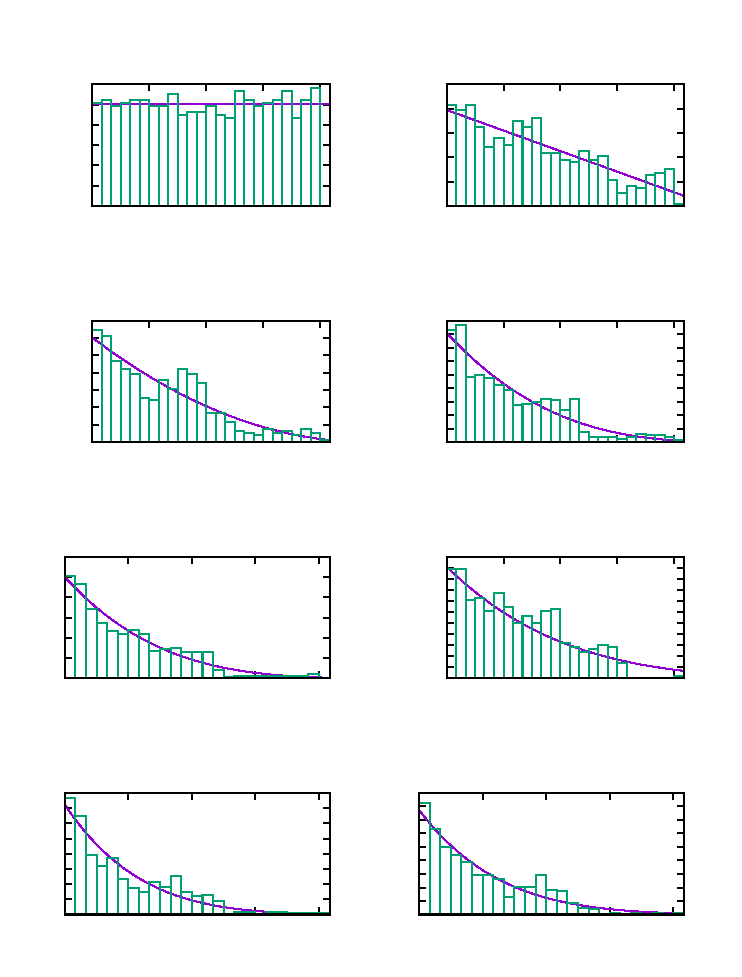
\includegraphics{figures/tex/histograms_I}}%
    \gplfronttext
  \end{picture}%
\endgroup

  \caption{histograms of the energy spacings for different spin lengths in the integrable case}\label{fig:hist_I0.5}
\end{figure}
If other parameters are chosen the match is even worse, especially for $\gamma = 1$ where for example the $j=1$ distribution almost perfectly matches a step function instead of a linear function, as can be seen in figure \ref{fig:hist_I1}.
Observing the spacing as a function of the engery where it ocurs can not only explain this behaviour, it also shows why the generalized formula \eqref{eq:p_n-I} might not be the best way to describe the energy spacings.
Depicted in figure \ref{fig:dE_I} are the energy spacings $\Delta \epsilon_i = \epsilon_i - \epsilon_{i-1}$ against $\epsilon_i$ and a clear structure is visible.
Three bands can be distinguished which originate from the independent threedimensional subspaces, that the hilbertspace collapses into in the integrable case.
These bands are each partwise linear with a general triangular structure.
In the case of $\gamma = 1$ two of these bands overlap exactly and there are no bends, so that only triangular bands, the density of which is apparently a step function.
For other parameter choices the triangular bands have bends somewhere along the slopes and (in the case of $j = 1$) there are three distinguished bands.
These two properties create a fairly linear slope, so equation \eqref{eq:p_n-I} is applicable.
Also $\nu = 1$ is necessary to for the unusual step distribution.

